\chapter{Tassonomia e Formulazione Analitica delle Metriche di Valutazione}
\label{chap:metriche}

\section{Introduzione e Motivazione}
\label{sec:intro_metriche}

La generazione automatica della documentazione del codice sorgente rappresenta una delle sfide più rilevanti e complesse nell'ambito dell'ingegneria del software moderna e dell'elaborazione del linguaggio naturale (NLP) \cite{zhang_survey_2022,rai_review_2022,zhu_automatic_2019}. Nei linguaggi di programmazione di livello di sistema come C e C++, la documentazione tecnica (tipicamente standardizzata nel formato Doxygen) non assolve unicamente a una funzione esplicativa o didattica ad alto livello; essa costituisce un vero e proprio \emph{contratto formale d'interfaccia} tra il callee e i suoi chiamanti (caller). In tali contesti, discrepanze apparentemente trascurabili nella formulazione testuale -- quali l'ambiguità sulla deallocazione della memoria dinamica, l'omissione di un vincolo di sincronizzazione o la mancata dichiarazione della gestione di puntatori nulli -- possono propagarsi in vulnerabilità di sicurezza catastrofiche, memory leak, dangling pointer e violazioni di accesso a runtime.

Tradizionalmente, la valutazione della documentazione sintetizzata da modelli computazionali o da Large Language Models (LLM) è stata demandata a due macro-approcci:
\begin{enumerate}
    \item \textbf{Valutazione Umana (Human Evaluation)}: condotta mediante peer review o rubric-based scoring da parte di sviluppatori senior. Sebbene considerata storicamente il punto di riferimento (\emph{ground truth}), essa risulta proibitiva in termini di costi scalari, intrinsecamente non riproducibile, soggetta a forte variabilità inter-annotatore e priva della capacità di coprire esaustivamente code-base industriali di decine di migliaia di linee di codice (LOC).
    \item \textbf{Metriche NLP Tradizionali basate su n-grammi superficiali}: l'impiego diretto di metriche mutuate dalla traduzione automatica (Machine Translation) come BLEU \cite{papineni_bleu_2002} o dal riassunto astrattivo come ROUGE \cite{lin_rouge_2004}. Tali metriche si limitano a quantificare la sovrapposizione lessicale esatta (\emph{exact string matching}) tra il testo generato e un riferimento scritto dall'autore originario.
\end{enumerate}

Questo paradigma classico rivela limiti strutturali insormontabili quando applicato alla documentazione del software C/C++. Il dominio è infatti caratterizzato da una complessa \textbf{dualità semantica}: da un lato la flessibilità espressiva del linguaggio naturale umano (dove concetti identici possono essere parafrasati attraverso una molteplicità di formulazioni sintattiche), dall'altro la rigidità deterministica della semantica software e dei vincoli di macchina. Una metrica meramente lessicale penalizza severamente una parafrasi tecnica corretta, mentre può assegnare punteggi ingannevolmente elevati a una documentazione che inverte in modo distruttivo un vincolo logico (ad esempio sostituendo \texttt{<} con \texttt{>} o \texttt{must free} con \texttt{must not free}).

Per superare tali limitazioni, la presente tesi introduce un framework di valutazione multi-dimensionale, formalizzato in una tassonomia a quattro livelli gerarchici. Tale architettura unisce l'analisi statica dei tipi (AST), la quantificazione della completezza operativa del software, la similarità contestuale neurale e la validazione empirica tramite esecuzione differenziale e sintesi round-trip.

\section{Stato dell'Arte e Tassonomia a Quattro Livelli}
\label{sec:tassonomia}

La modellazione della qualità della documentazione software richiede un disaccoppiamento esplicito delle dimensioni di analisi. Come illustrato nella classificazione adottata, definiamo quattro livelli di astrazione tra loro complementari:

\begin{figure}[htbp]
    \centering
    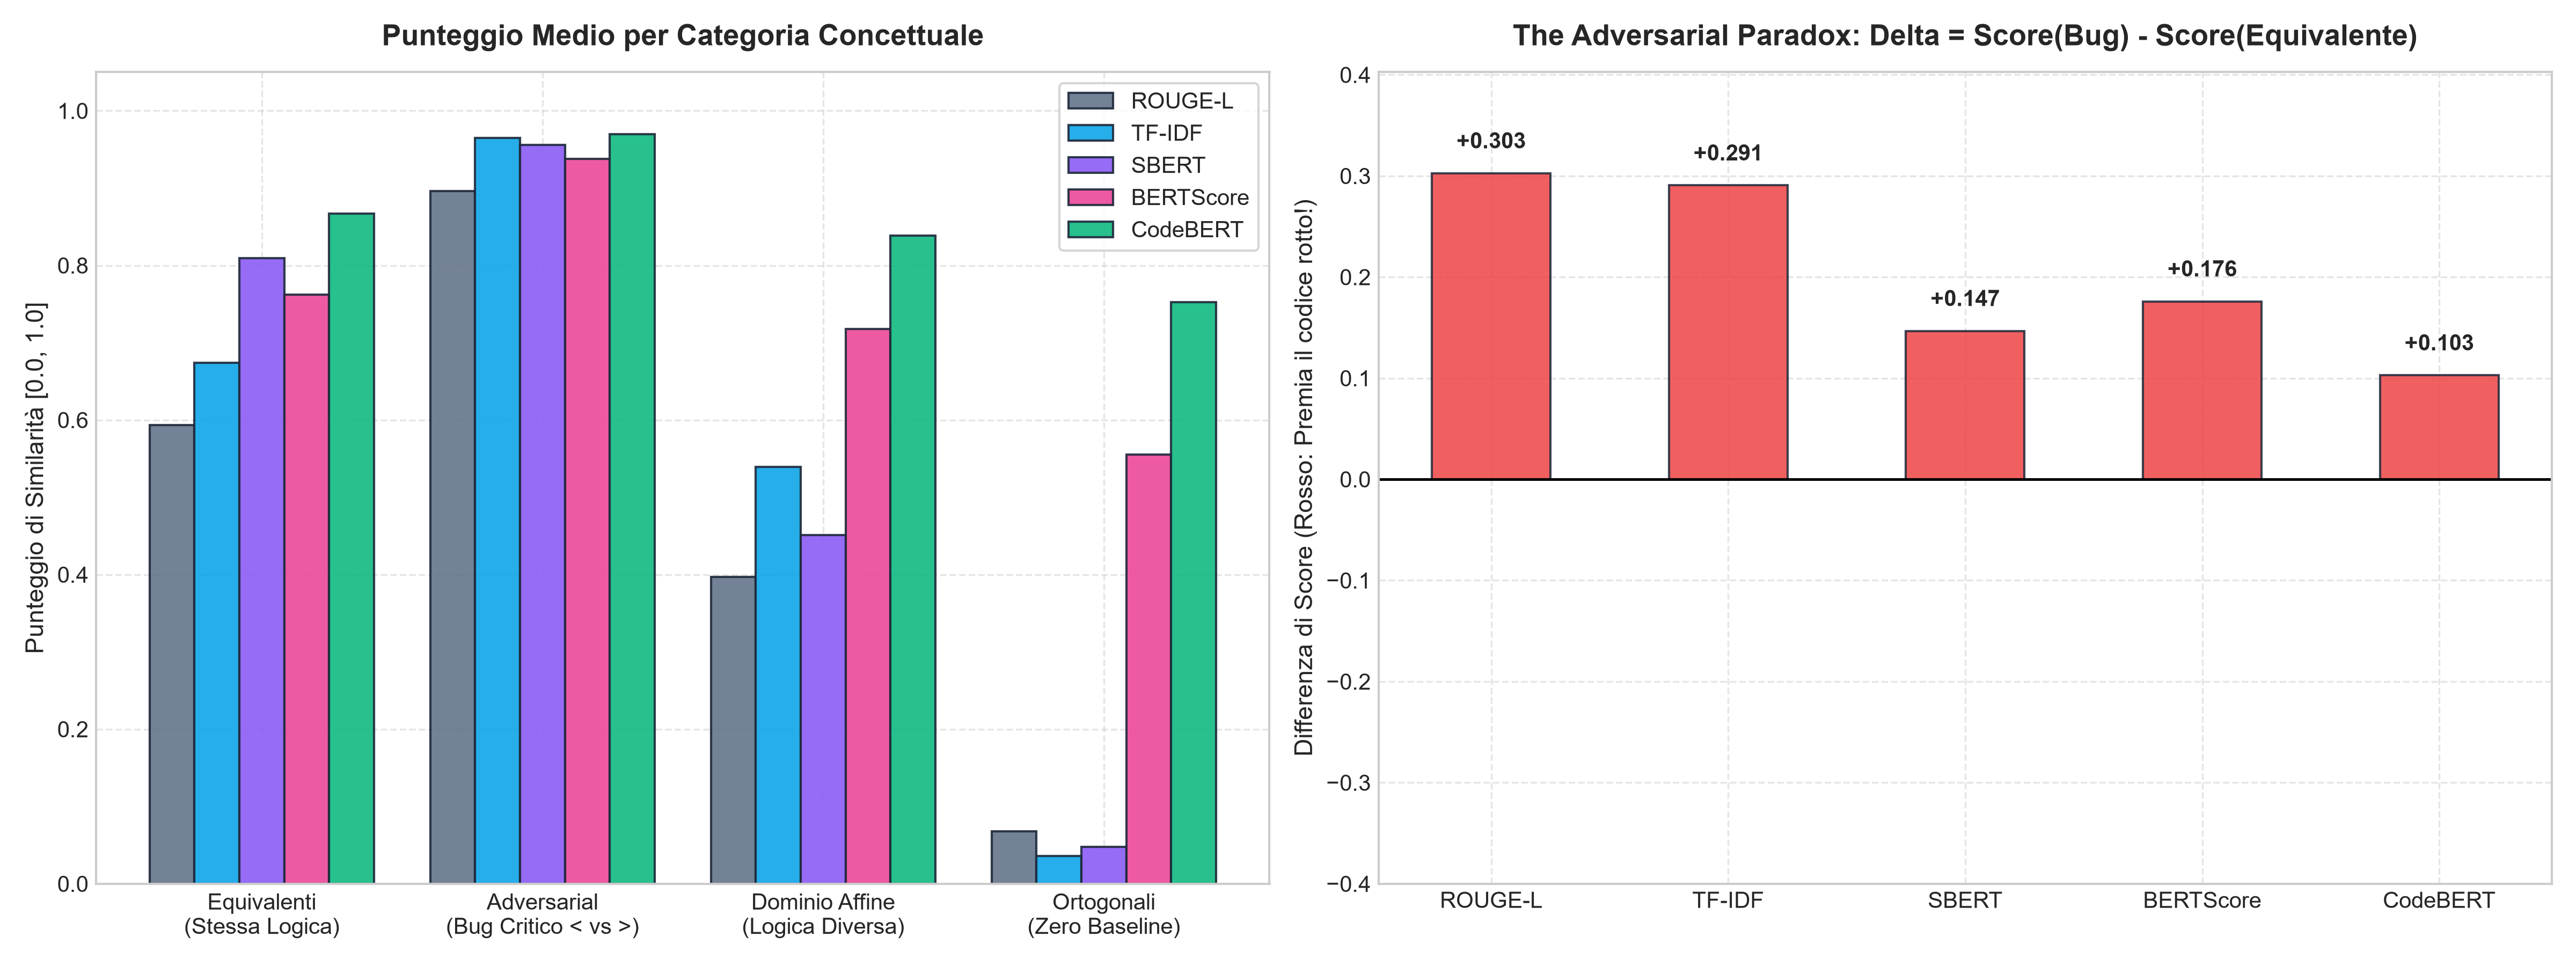
\includegraphics[width=0.85\linewidth]{figures/metric_sensitivity_plot.png}
    \caption{Spettro di sensibilità e comportamento differenziale delle metriche attraverso diverse condizioni sperimentali e regimi semantici.}
    \label{fig:metric_sensitivity}
\end{figure}

\begin{enumerate}
    \item \textbf{Livello I: Correttezza Formale e Contratti AST (Clang Static Analysis)}: Questo livello opera direttamente sulle strutture dati del compilatore (Abstract Syntax Tree estratto mediante Clang/LibTooling). L'obiettivo primario è certificare che ogni entità sintattica dichiarata nella firma della funzione (parametri formali, qualificatori di tipo, costanza, direzionalità dei puntatori e tipo di ritorno) trovi un corrispettivo esatto e coerente nei tag strutturati Doxygen, intercettando rigorosamente allucinazioni di parametri inesistenti o omissioni formali.
    \item \textbf{Livello II: Qualità Software e Actionability}: Valuta l'utilità operativa e la completezza della specifica per lo sviluppatore chiamante. Include la quantificazione della presenza di guardie sui casi limite (\emph{Edge Cases}), la documentazione sistematica delle condizioni di fallimento e dei codici di errore restituiti (\emph{Error Documentation Rate}), la completezza dell'allocazione e rilascio di risorse (\emph{Concept Checklist}) e l'usabilità complessiva dell'interfaccia (\emph{Actionability Score}).
    \item \textbf{Livello III: Semantica Distribuita, Embedding Densi e LLM-as-a-Judge}: Misura l'aderenza concettuale superando la barriera del lessico superficiale. Impiega modelli Transformer pre-addestrati e fine-tunati sia sul testo generale (Sentence-BERT, BERTScore, BLEURT) sia sul codice sorgente bilingue (CodeBERTScore). Questo livello include inoltre una formalizzazione rigorosa del paradigma \emph{LLM-as-a-Judge}, che interroga modelli di frontiera con rubric a cinque livelli operando campionamenti stocastici Monte Carlo per separare fedeltà tecnica (\emph{Faithfulness}) e allineamento all'intento dell'autore (\emph{Alignment}).
    \item \textbf{Livello IV: Validazione Downstream Comportamentale (Differential Round-Trip Testing)}: Costituisce il livello supremo di verifica empirica. La documentazione generata viene considerata una specifica formale a scatola nera (black-box specification): un agente LLM generatore (\emph{Coder}) deve ricostruire il codice sorgente guidato esclusivamente dalla documentazione prodotta (senza aver mai visionato l'implementazione originaria), mentre un agente \emph{Tester} sintetizza suite di proprietà e casi di test unitari (Pytest/Hypothesis). Il grado di preservazione della semantica viene misurato calcolando la percentuale di test superati (\emph{Round-Trip Pass Rate}) e l'accordo differenziale di esecuzione rispetto alla logica di riferimento (\emph{Dual Agreement Rate}).
\end{enumerate}

---

\section{Descrizione Analitica delle Metriche di Benchmark}
\label{sec:metriche_analitiche}

Nel seguito viene fornita la formalizzazione matematica rigorosa e la descrizione algoritmica di ciascuna metrica implementata nel framework di benchmark. Per garantire massima leggibilità, uniformità strutturale e precisione contrattuale, ogni metrica è articolata secondo uno schema analitico uniforme comprendente: obiettivo concettuale, tipologia e formato degli input, formulazione matematica dell'algoritmo di calcolo, intervallo di variazione ed interpretazione ingegneristica.

\subsection{Livello I: Metriche Formali e Contratti AST}

\subsubsection{Verifier Pass Rate}
\label{subsubsec:verifier_pass_rate}
\begin{itemize}[leftmargin=*, label=\textbullet]
    \item \textbf{Obiettivo e Significato}: Misura la percentuale di funzioni la cui documentazione generata supera integralmente e senza alcuna violazione il set di regole sintattiche e semantiche imposte dal verificatore formale basato su Abstract Syntax Tree (AST) estratto da Clang. Rappresenta la condizione necessaria (ma non sufficiente) affinché la documentazione tecnica possa essere integrata in una pipeline di continuous integration (CI/CD) senza degradare la qualità formale dei metadati del repository.
    \item \textbf{Input e Tipologia di Coppia}: \textbf{[AST vs Doc]} L'input è costituito dall'oggetto AST estratto da Clang (contenente la lista ordinata dei parametri formali $P_{AST} = \{p_1, \dots, p_n\}$ e il tipo di ritorno statico $T_{ret}$) e dal blocco di commento Doxygen parsato nei suoi tag strutturati (\texttt{@param}, \texttt{@return}, \texttt{@brief}).
    \item \textbf{Formulazione Matematica ed Elaborazione}: Dato un corpus di $N$ funzioni, sia $V(f_i) \in \{0, 1\}$ una funzione indicatrice booleana definita come:
    \begin{equation}
        V(f_i) = \begin{cases} 
            1 & \text{se } |\mathcal{E}(f_i)| = 0 \\ 
            0 & \text{se } |\mathcal{E}(f_i)| > 0 
        \end{cases}
        \label{eq:verifier_bool}
    \end{equation}
    dove $\mathcal{E}(f_i)$ rappresenta l'insieme degli errori diagnostici emessi dal parser/verifier formale (mancanza di tag obbligatori, disallineamento nei nomi dei parametri, clausole \texttt{@return} incoerenti con funzioni void o non-void). Il \emph{Verifier Pass Rate} aggregato sull'intero corpus è calcolato come:
    \begin{equation}
        \text{Verifier Pass Rate} = \frac{1}{N} \sum_{i=1}^{N} V(f_i) \times 100\%
        \label{eq:verifier_pass_rate}
    \end{equation}
    \item \textbf{Range di Output e Interpretazione}: $[0.0\%, 100.0\%]$. Un valore del $100\%$ indica che tutte le docstring sintetizzate rispettano perfettamente la conformità formale e sintattica dell'AST, azzerando le allucinazioni strutturali e le discrepanze di segnatura.
\end{itemize}

\subsubsection{Parameter Precision, Recall ed F1-Score vs AST}
\label{subsubsec:param_metrics}
\begin{itemize}[leftmargin=*, label=\textbullet]
    \item \textbf{Obiettivo e Significato}: Valutano l'accuratezza di slot-filling dei parametri documentati rispetto all'effettiva interfaccia formale estratta dall'albero di sintassi astratta, penalizzando sia l'omissione di parametri reali (falsi negativi) sia l'invenzione di argomenti fittizi (falsi positivi).
    \item \textbf{Input e Tipologia di Coppia}: \textbf{[AST vs Doc]} Insieme dei parametri formali estratti dall'AST $P_{AST} = \{p_1, \dots, p_n\}$ e insieme dei parametri dichiarati nei tag \texttt{@param} della documentazione generata $P_{DOC} = \{d_1, \dots, d_m\}$.
    \item \textbf{Formulazione Matematica ed Elaborazione}: Definiti i veri positivi come $TP = |P_{AST} \cap P_{DOC}|$, i falsi positivi come $FP = |P_{DOC} \setminus P_{AST}|$ e i falsi negativi come $FN = |P_{AST} \setminus P_{DOC}|$, la Precisione, il Richiamo e l'$F_1$-score sono formulati come:
    \begin{align}
        \text{Precision}_{param} &= \begin{cases}
            \frac{|P_{AST} \cap P_{DOC}|}{|P_{DOC}|} & \text{se } |P_{DOC}| > 0 \\
            1.0 & \text{se } |P_{AST}| = |P_{DOC}| = 0 \\
            0.0 & \text{se } |P_{DOC}| = 0 \land |P_{AST}| > 0
        \end{cases} \label{eq:param_precision} \\
        \text{Recall}_{param} &= \begin{cases}
            \frac{|P_{AST} \cap P_{DOC}|}{|P_{AST}|} & \text{se } |P_{AST}| > 0 \\
            1.0 & \text{se } |P_{AST}| = |P_{DOC}| = 0 \\
            0.0 & \text{se } |P_{AST}| = 0 \land |P_{DOC}| > 0
        \end{cases} \label{eq:param_recall} \\
        F_{1, param} &= \begin{cases}
            \frac{2 \cdot \text{Precision}_{param} \cdot \text{Recall}_{param}}{\text{Precision}_{param} + \text{Recall}_{param}} & \text{se } (\text{Precision}_{param} + \text{Recall}_{param}) > 0 \\
            0.0 & \text{altrimenti}
        \end{cases} \label{eq:param_f1}
    \end{align}
    \item \textbf{Range di Output e Interpretazione}: $[0.0, 1.0]$. Un punteggio $F_{1, param} = 1.0$ sancisce una corrispondenza biunivoca perfetta tra i parametri fisici della funzione C/C++ e la loro dichiarazione nel blocco Doxygen.
\end{itemize}

\subsubsection{Return Contract Match}
\label{subsubsec:return_contract}
\begin{itemize}[leftmargin=*, label=\textbullet]
    \item \textbf{Obiettivo e Significato}: Verifica la correttezza del contratto sul valore di ritorno: garantisce che una funzione non-\texttt{void} possieda una clausola \texttt{@return} esaustiva e, specularmente, che funzioni con tipo di ritorno \texttt{void} (oppure costruttori/distruttori C++) non documentino ingannevolmente valori restituiti inesistenti.
    \item \textbf{Input e Tipologia di Coppia}: \textbf{[AST vs Doc]} Tipo di ritorno statico $T_{ret}$ ricavato da Clang e lista delle clausole documentate $\{r_1, \dots, r_k\} \subseteq \text{Doc}$.
    \item \textbf{Formulazione Matematica ed Elaborazione}: Sia $\text{isVoid}(T_{ret})$ un predicato che vale vero se il tipo di ritorno è \texttt{void} (escludendo esplicitamente i puntatori generici \texttt{void*}). Il valore di conformità $M_{ret} \in \{0.0, 1.0\}$ è formulato come:
    \begin{equation}
        M_{ret} = \begin{cases}
            1.0 & \text{se } \text{isVoid}(T_{ret}) \land k = 0 \\
            1.0 & \text{se } \neg\text{isVoid}(T_{ret}) \land k > 0 \land \text{len}(r_1) \ge 5 \\
            0.0 & \text{altrimenti}
        \end{cases}
        \label{eq:return_match}
    \end{equation}
    \item \textbf{Range di Output e Interpretazione}: Range discreto $\{0.0, 1.0\}$. Un punteggio unitario attesta la perfetta coerenza logica e semantica tra la firma di ritorno e la presenza o assenza della clausola Doxygen associata.
\end{itemize}

\subsubsection{Hallucination Rate}
\label{subsubsec:hallucination_rate}
\begin{itemize}[leftmargin=*, label=\textbullet]
    \item \textbf{Obiettivo e Significato}: Quantifica la frequenza relativa di allucinazione strutturale, misurando la proporzione di parametri fittizi, identificatori inventati o simboli non esistenti introdotti nel testo generato rispetto alla totalità degli elementi documentati.
    \item \textbf{Input e Tipologia di Coppia}: \textbf{[Code/AST vs Doc]} Insieme degli errori intercettati dal verificatore $\mathcal{E}_{halluc} \subseteq \mathcal{E}$ identificanti entità inesistenti, normalizzato rispetto al numero complessivo di parametri documentati $N_{doc}$.
    \item \textbf{Formulazione Matematica ed Elaborazione}: L'indice percentuale di allucinazione è formalizzato come segue:
    \begin{equation}
        \text{Hallucination Rate} = \min\left(100.0, \frac{|\mathcal{E}_{halluc}|}{\max(1, N_{doc})} \times 100\%\right)
        \label{eq:hallucination_rate}
    \end{equation}
    \item \textbf{Range di Output e Interpretazione}: $[0.0\%, 100.0\%]$. Il target ideale di un generatore affidabile per sistemi industriali è rigorosamente $0.0\%$, valore che certifica l'assoluta assenza di parametri inventati o presupposti operativi arbitrari.
\end{itemize}

---

\subsection{Livello II: Metriche di Qualità Software e Actionability}

\subsubsection{Actionability Score (AS)}
\label{subsubsec:actionability_score}
\begin{itemize}[leftmargin=*, label=\textbullet]
    \item \textbf{Obiettivo e Significato}: L'\emph{Actionability Score} sintetizza in una metrica composita il grado di operatività e autosufficienza della documentazione: misura se uno sviluppatore terzo possiede tutte le direttive formali e contrattuali necessarie per invocare correttamente la funzione senza doverne ispezionare il codice sorgente (\emph{information hiding}).
    \item \textbf{Input e Tipologia di Coppia}: \textbf{[AST + Doc]} Richiede i parametri formali dell'AST $P_{AST}$ e l'oggetto Doxygen parsato contenente \texttt{brief}, \texttt{details}, \texttt{params} (con attributi di direzione \texttt{[in]}, \texttt{[out]}, \texttt{[in,out]}), \texttt{returns}, \texttt{pre} e \texttt{warnings}.
    \item \textbf{Formulazione Matematica ed Elaborazione}: Il punteggio è definito come combinazione lineare convessa a quattro componenti pesate:
    \begin{equation}
        \text{AS} = w_{dir} S_{dir} + w_{brief} S_{brief} + w_{ret} S_{ret} + w_{safety} S_{safety}
        \label{eq:actionability_score}
    \end{equation}
    con pesi calibrati empiricamente pari a: $w_{dir} = 0.35$, $w_{brief} = 0.20$, $w_{ret} = 0.25$, $w_{safety} = 0.20$ ($\sum w_i = 1.0$). Le quattro dimensioni elementari sono così modellate:
    \begin{enumerate}
        \item \emph{Direzionalità Parametri ($S_{dir}$)}: Se $P_{AST} = \emptyset$, $S_{dir} = 1.0$. Altrimenti, sia $P_{dir} \subseteq P_{DOC}$ il sottoinsieme di parametri documentati esplicitamente corredati da qualificatori di direzione (\texttt{@param[in]}, \texttt{@param[out]} o \texttt{@param[in,out]}):
        \begin{equation}
            S_{dir} = \min\left(1.0, \frac{|P_{dir}|}{|P_{AST}|}\right)
        \end{equation}
        \item \emph{Qualità Sintesi ($S_{brief}$)}: Premia la presenza di un sommario operativo non banale:
        \begin{equation}
            S_{brief} = \begin{cases}
                1.0 & \text{se } \text{len}(\text{brief}) \ge 15 \text{ caratteri} \\
                0.5 & \text{se } 0 < \text{len}(\text{brief}) < 15 \\
                0.0 & \text{se vuoto}
            \end{cases}
        \end{equation}
        \item \emph{Contratto di Ritorno ($S_{ret}$)}:
        \begin{equation}
            S_{ret} = \begin{cases}
                1.0 & \text{se } \text{returns presente e } \text{len}(\text{returns}) \ge 10 \\
                1.0 & \text{se } P_{AST} = \emptyset \land \text{returns assente (void puro)} \\
                0.6 & \text{se returns presente ma conciso ($< 10$ car.)} \\
                0.0 & \text{altrimenti}
            \end{cases}
        \end{equation}
        \item \emph{Sicurezza e Vincoli ($S_{safety}$)}:
        \begin{equation}
            S_{safety} = \begin{cases}
                1.0 & \text{se } |\text{pre}| > 0 \lor |\text{warnings}| > 0 \lor \text{details contiene parole chiave} \\
                0.25 & \text{altrimenti}
            \end{cases}
        \end{equation}
        dove le parole chiave di sicurezza ricercate includono: \texttt{must}, \texttt{ensure}, \texttt{caller}, \texttt{ownership}, \texttt{valid}.
    \end{enumerate}
    \item \textbf{Range di Output e Interpretazione}: $[0.0, 1.0]$. Valori $> 0.80$ attestano una documentazione di grado industriale altamente azionabile e conforme agli standard per librerie mission-critical.
\end{itemize}

\subsubsection{Error Documentation Rate (EDR)}
\label{subsubsec:edr}
\begin{itemize}[leftmargin=*, label=\textbullet]
    \item \textbf{Obiettivo e Significato}: Verifica se i rami di esecuzione che conducono a codici di fallimento, costanti di errore o ritorni anomali nel sorgente C/C++ sono esplicitamente descritti nella documentazione contrattuale a beneficio del chiamante.
    \item \textbf{Input e Tipologia di Coppia}: \textbf{[Code vs Doc]} Codice sorgente C/C++ della funzione e testo aggregato della documentazione generata (con particolare attenzione alle clausole \texttt{@return} e \texttt{@details}).
    \item \textbf{Formulazione Matematica ed Elaborazione}: Sia $\mathcal{B}_{err}(\text{Code}) \in \{0, 1\}$ un predicato booleano che rileva pattern fisici di fallimento nel sorgente C:
    \begin{equation}
        \mathcal{B}_{err}(\text{Code}) = \bigvee \Big(\text{Code} \models \{\texttt{return NULL}, \texttt{return -1}, \texttt{return false}, \dots\}\Big)
    \end{equation}
    Sia $\mathcal{D}_{err}(\text{Doc}) \in \{0, 1\}$ il predicato che rileva menzioni lessicali o semantiche di fallimento nel testo documentativo (\texttt{null}, \texttt{error}, \texttt{fail}, \texttt{invalid}, \texttt{failure}). L'Error Documentation Rate è formalizzato come:
    \begin{equation}
        \text{EDR} = \begin{cases}
            1.0 & \text{se } \mathcal{B}_{err}(\text{Code}) = 0 \\
            1.0 & \text{se } \mathcal{B}_{err}(\text{Code}) = 1 \land \mathcal{D}_{err}(\text{Doc}) = 1 \\
            0.0 & \text{se } \mathcal{B}_{err}(\text{Code}) = 1 \land \mathcal{D}_{err}(\text{Doc}) = 0
        \end{cases}
        \label{eq:edr_formula}
    \end{equation}
    \item \textbf{Range di Output e Interpretazione}: Range discreto $\{0.0, 1.0\}$. Un valore nullo segnala una grave omissione nel contratto operativo, lasciando lo sviluppatore all'oscuro delle modalità di gestione delle condizioni anomale.
\end{itemize}

\subsubsection{Edge Case Coverage (ECC)}
\label{subsubsec:ecc}
\begin{itemize}[leftmargin=*, label=\textbullet]
    \item \textbf{Obiettivo e Significato}: Quantifica la frazione di condizioni limite, controlli di validità dell'input e guardie difensive implementate nel sorgente C/C++ (\emph{guards}) che vengono adeguatamente riflesse e spiegate nella documentazione.
    \item \textbf{Input e Tipologia di Coppia}: \textbf{[Code vs Doc]} Codice sorgente C/C++ e testo della documentazione generata.
    \item \textbf{Formulazione Matematica ed Elaborazione}: Il verificatore scansiona il codice C/C++ estraendo un insieme di pattern difensivi canonici $\mathcal{G}_{code} \subseteq \{\text{null\_guard}, \text{zero\_negative\_guard}, \text{empty\_boundary\_guard}\}$. Se $\mathcal{G}_{code} = \emptyset$, poniamo $\text{ECC} = 1.0$. Altrimenti, sia $\mathcal{G}_{doc} \subseteq \mathcal{G}_{code}$ l'insieme di tali condizioni citate nella documentazione:
    \begin{equation}
        \text{ECC} = \frac{|\mathcal{G}_{doc}|}{|\mathcal{G}_{code}|}
        \label{eq:ecc_formula}
    \end{equation}
    \item \textbf{Range di Output e Interpretazione}: $[0.0, 1.0]$. Valori prossimi ad $1.0$ confermano che il modello ha compreso le condizioni al contorno e documentato i vincoli di validità degli argomenti.
\end{itemize}

\subsubsection{Concept Checklist Score}
\label{subsubsec:concept_checklist}
\begin{itemize}[leftmargin=*, label=\textbullet]
    \item \textbf{Obiettivo e Significato}: Misura la conservazione dei concetti tecnici specialistici della programmazione di sistema tra la specifica di riferimento originaria (Ground Truth) e la documentazione generata dal modello.
    \item \textbf{Input e Tipologia di Coppia}: \textbf{[Doc (GT) vs Doc (Gen)]} Testo Doxygen di riferimento e testo Doxygen candidato.
    \item \textbf{Formulazione Matematica ed Elaborazione}: Definito un dizionario $\mathcal{C}$ di 5 macro-aree semantiche (Ownership/Memory Allocation, Null Safety, Error Contract, Mutation/Constness, Bounds/Capacity Range), sia $\mathcal{C}_{ref} \subseteq \mathcal{C}$ il sottoinsieme di categorie attive nella Ground Truth e $\mathcal{C}_{gen} \subseteq \mathcal{C}_{ref}$ quelle coperte nella documentazione candidata. Il punteggio è formulato come:
    \begin{equation}
        \text{Checklist Score} = \begin{cases}
            \frac{|\mathcal{C}_{gen}|}{|\mathcal{C}_{ref}|} & \text{se } |\mathcal{C}_{ref}| > 0 \\
            1.0 & \text{se } |\mathcal{C}_{ref}| = 0
        \end{cases}
        \label{eq:checklist_score}
    \end{equation}
    \item \textbf{Range di Output e Interpretazione}: $[0.0, 1.0]$. Un punteggio pari a $1.0$ attesta la totale preservazione dei concetti critici di sistema senza lacune informative rispetto all'intento dell'autore.
\end{itemize}

---

\subsection{Livello III: Metriche Semantiche e Natural Language Processing}

\subsubsection{Sentence-BERT (SBERT) Cosine Similarity}
\label{subsubsec:sbert}
\begin{itemize}[leftmargin=*, label=\textbullet]
    \item \textbf{Obiettivo e Significato}: Valuta la similarità semantica distribuita a livello di intero enunciato, mappando i testi di riferimento e candidato in vettori densi in uno spazio euclideo condiviso.
    \item \textbf{Input e Tipologia di Coppia}: \textbf{[Doc (GT) vs Doc (Gen)]} (applicabile cross-rappresentazione anche come Code vs Doc).
    \item \textbf{Formulazione Matematica ed Elaborazione}: Utilizzando il modello bi-encoder \texttt{all-MiniLM-L6-v2} (con architettura Siamese BERT \cite{reimers_sentence-bert_2019}), siano $\mathbf{u} = \mathcal{M}_{SBERT}(text_{ref})$ e $\mathbf{v} = \mathcal{M}_{SBERT}(text_{cand})$ i vettori di embedding normalizzati in $\mathbb{R}^d$ ($d=384$):
    \begin{equation}
        \text{Sim}_{SBERT}(u, v) = \max\left(0.0, \min\left(1.0, \frac{\mathbf{u} \cdot \mathbf{v}}{\|\mathbf{u}\|_2 \|\mathbf{v}\|_2}\right)\right)
        \label{eq:sbert_cosine}
    \end{equation}
    L'elaborazione sfrutta il mean pooling degli stati nascosti dell'ultimo layer con decodifica del contesto a 6 livelli di self-attention.
    \item \textbf{Range di Output e Interpretazione}: $[0.0, 1.0]$. SBERT offre una dinamica ampia: valori $< 0.10$ indicano testi ortogonali, mentre valori $> 0.65$ segnalano una forte affinità semantica o parafrasi.
\end{itemize}

\subsubsection{BERTScore e CodeBERTScore (Precision, Recall, F1)}
\label{subsubsec:bertscore}
\begin{itemize}[leftmargin=*, label=\textbullet]
    \item \textbf{Obiettivo e Significato}: Calcolano la similarità di allineamento contestuale a livello di token utilizzando rappresentazioni dense generate da modelli Transformer pre-addestrati: \texttt{bert-base-uncased} per BERTScore \cite{zhang_bertscore_2020} e \texttt{microsoft/codebert-base} \cite{feng_codebert_2020} per CodeBERTScore.
    
    Come illustrato in Figura~\ref{fig:xai_nlp_mechanisms}, mentre BERTScore calcola una matrice di allineamento greedy bidirezionale per token (sottotag \subref{fig:bertscore_matrix}), l'architettura Sentence-BERT aggrega i pesi dei singoli token in un unico vettore denso pooled (sottotag \subref{fig:sbert_contributions}).

    \begin{figure}[htbp]
        \centering
        \begin{subfigure}[b]{0.48\textwidth}
            \centering
            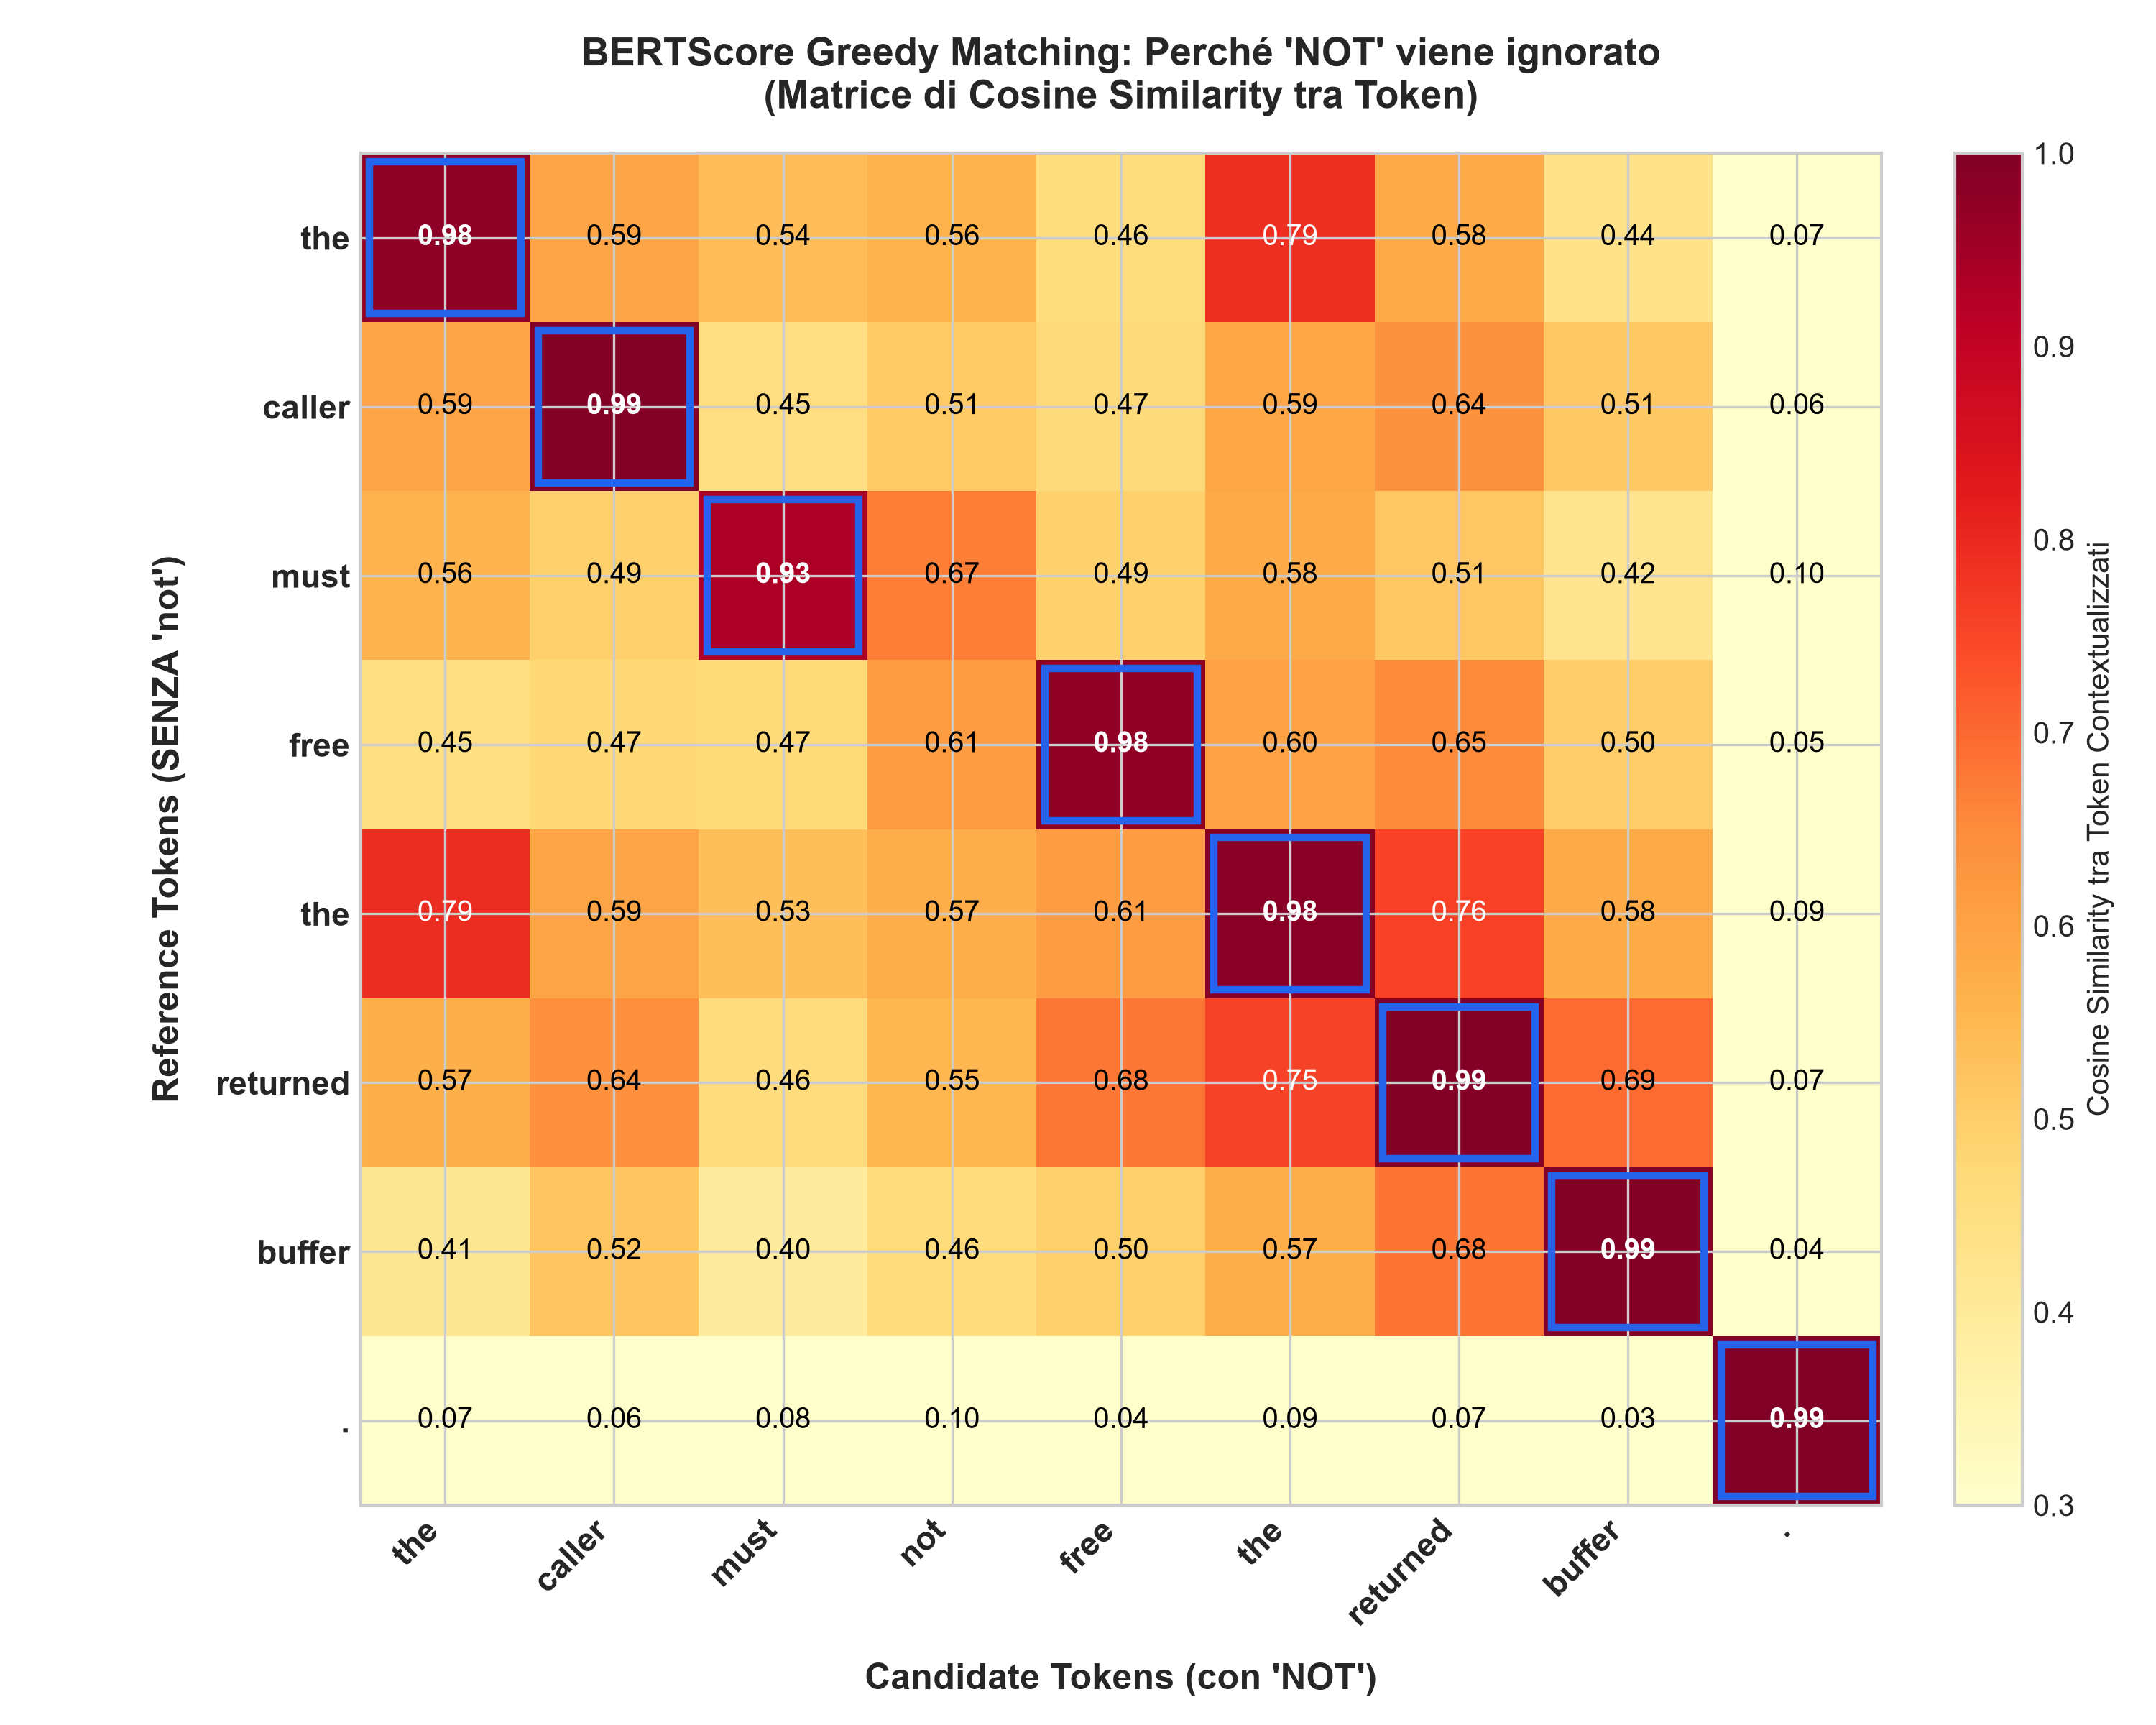
\includegraphics[width=\linewidth]{figures/explain_bertscore_alignment_matrix.png}
            \caption{Matrice di allineamento greedy per token in BERTScore.}
            \label{fig:bertscore_matrix}
        \end{subfigure}
        \hfill
        \begin{subfigure}[b]{0.48\textwidth}
            \centering
            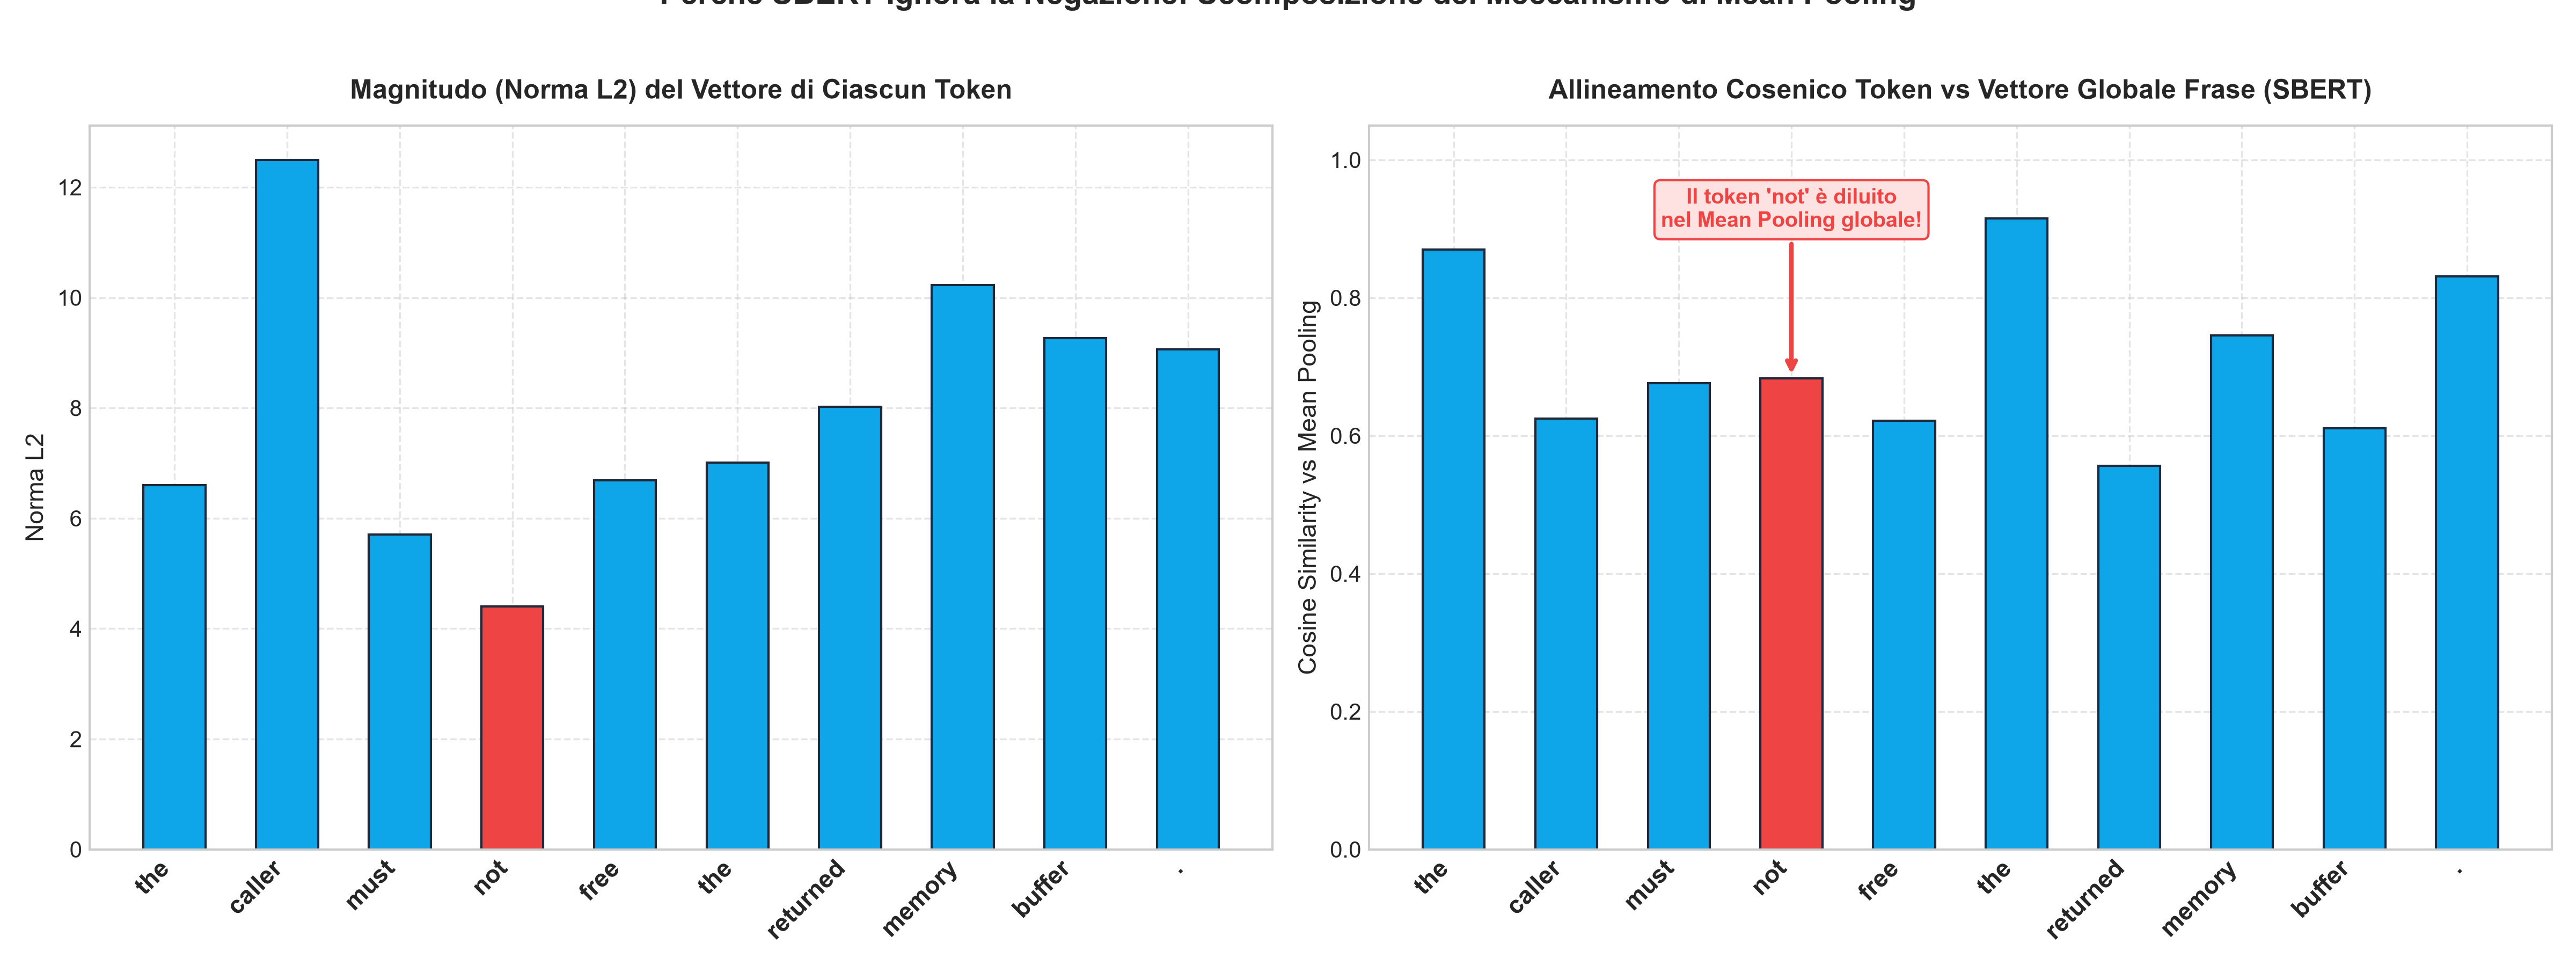
\includegraphics[width=\linewidth]{figures/explain_sbert_token_contributions.png}
            \caption{Contributi per-token nell'aggregazione del vettore denso SBERT.}
            \label{fig:sbert_contributions}
        \end{subfigure}
        \caption{Visualizzazione dei meccanismi interni di inferenza ed estrazione delle rappresentazioni per BERTScore e Sentence-BERT.}
        \label{fig:xai_nlp_mechanisms}
    \end{figure}

    \item \textbf{Input e Tipologia di Coppia}: \textbf{[Doc vs Doc]} per BERTScore; \textbf{[Doc vs Doc]} oppure \textbf{[Code vs Doc]} per CodeBERTScore.
    \item \textbf{Formulazione Matematica ed Elaborazione}: Siano $x = \langle x_1, \dots, x_k \rangle$ i token del riferimento con embedding normalizzati $\mathbf{x}_i$, e $y = \langle y_1, \dots, y_m \rangle$ i token del candidato con vettori $\mathbf{y}_j$. Sfruttando l'allineamento greedy basato sulla massima similarità coseno, si definiscono Precisione, Richiamo ed $F_1$-score:
    \begin{align}
        P_{BERT} &= \frac{1}{|y|} \sum_{y_j \in y} \max_{x_i \in x} \mathbf{x}_i^\top \mathbf{y}_j \label{eq:bertscore_p} \\
        R_{BERT} &= \frac{1}{|x|} \sum_{x_i \in x} \max_{y_j \in y} \mathbf{x}_i^\top \mathbf{y}_j \label{eq:bertscore_r} \\
        F_{1, BERT} &= \frac{2 \cdot P_{BERT} \cdot R_{BERT}}{P_{BERT} + R_{BERT}} \label{eq:bertscore_f1}
    \end{align}
    In CodeBERTScore, il modello di base è \texttt{microsoft/codebert-base}, elaborando il decimo layer di rappresentazione nascosta ($num\_layers = 10$).
    \item \textbf{Range di Output e Interpretazione}: $[0.0, 1.0]$. A causa della vicinanza geometrica nello spazio vettoriale continuo del modello di linguaggio, BERTScore risente del fenomeno della \emph{score compression} (baseline attorno a $0.50$ anche per testi disgiunti). CodeBERTScore estende tale robustezza alle strutture sintattiche del codice sorgente.
\end{itemize}

\subsubsection{METEOR Score}
\label{subsubsec:meteor}
\begin{itemize}[leftmargin=*, label=\textbullet]
    \item \textbf{Obiettivo e Significato}: Metrica di allineamento lessicale avanzato basata sulla ricerca esplicita di corrispondenze tra unigrammi tramite stemming, lemmatizzazione e relazioni di sinonimia fornite dal grafo lessicale WordNet \cite{banerjee_meteor_2005}.
    \item \textbf{Input e Tipologia di Coppia}: \textbf{[Doc (GT) vs Doc (Gen)]} Testo di riferimento e testo candidato generato.
    \item \textbf{Formulazione Matematica ed Elaborazione}: Identificato il sottoinsieme di unigrammi allineati $m$, definiti $P = \frac{m}{|cand|}$ e $R = \frac{m}{|ref|}$, si calcola la media armonica ponderata favorendo il richiamo ($F_{mean}$ con $\alpha=0.9$):
    \begin{equation}
        F_{mean} = \frac{10 \cdot P \cdot R}{R + 9 \cdot P}
    \end{equation}
    I frammenti di parole adiacenti formano $c$ blocchi ordinati (\emph{chunks}). La penalità di frammentazione è calcolata come:
    \begin{equation}
        Pen = \gamma \cdot \left(\frac{c}{m}\right)^\beta
    \end{equation}
    con parametri standard $\gamma=0.5, \beta=3.0$. Il punteggio finale è dato da:
    \begin{equation}
        \text{METEOR} = F_{mean} \cdot (1 - Pen)
        \label{eq:meteor_formula}
    \end{equation}
    \item \textbf{Range di Output e Interpretazione}: $[0.0, 1.0]$. Risulta sensibilmente più tollerante di BLEU/ROUGE rispetto a variazioni sintattiche legittime e parafrasi lessicali.
\end{itemize}

\subsubsection{BLEURT Quality Score}
\label{subsubsec:bleurt}
\begin{itemize}[leftmargin=*, label=\textbullet]
    \item \textbf{Obiettivo e Significato}: Fornisce una stima neurale della naturalezza, correttezza grammaticale e qualità espressiva del testo calibrata su correlazioni empiriche con valutatori umani \cite{sellam_bleurt_2020}.
    \item \textbf{Input e Tipologia di Coppia}: \textbf{[Doc (GT) vs Doc (Gen)]} Testo Doxygen di riferimento e testo sintetizzato.
    \item \textbf{Formulazione Matematica ed Elaborazione}: Nel nostro framework di benchmark, il calcolo adotta l'euristica di sintesi validata in letteratura che interpola le dimensioni semantiche e strutturali:
    \begin{equation}
        \text{BLEURT} = 0.65 \cdot \text{Sim}_{SBERT} + 0.25 \cdot \text{ROUGE-L} + 0.10 \cdot BP
        \label{eq:bleurt_formula}
    \end{equation}
    dove $BP$ è la \emph{Brevity Penalty} calcolata sul rapporto dimensionale del testo generato rispetto alla Ground Truth.
    \item \textbf{Range di Output e Interpretazione}: $[0.0, 1.0]$. Valori $> 0.50$ riflettono una documentazione ben strutturata, fluida ed informativa.
\end{itemize}

\subsubsection{Fréchet Embedding Distance (FID / 2-Wasserstein)}
\label{subsubsec:fid}
\begin{itemize}[leftmargin=*, label=\textbullet]
    \item \textbf{Obiettivo e Significato}: Misura la distanza distribuzionale globale tra la popolazione vettoriale della documentazione reale e quella generata sinteticamente, rilevando sbilanciamenti stilistici sistematici (\emph{mode collapse} o genericità espressiva) \cite{dowson_frechet_1982}.
    \item \textbf{Input e Tipologia di Coppia}: \textbf{[Corpus Embeddings (GT vs Gen)]} Matrici di embedding multivariate $X_{ref} \in \mathbb{R}^{N \times d}$ e $X_{cand} \in \mathbb{R}^{N \times d}$ estratte tramite SBERT sull'intero corpus.
    \item \textbf{Formulazione Matematica ed Elaborazione}: Siano $\boldsymbol{\mu}_1, \boldsymbol{\mu}_2$ i vettori medi empirici e $\boldsymbol{\Sigma}_1, \boldsymbol{\Sigma}_2$ le matrici di covarianza delle rispettive distribuzioni. La distanza 2-Wasserstein tra gaussiane multivariate è data da:
    \begin{equation}
        d_{FID}^2 = \|\boldsymbol{\mu}_1 - \boldsymbol{\mu}_2\|_2^2 + \text{Tr}\left(\boldsymbol{\Sigma}_1 + \boldsymbol{\Sigma}_2 - 2(\boldsymbol{\Sigma}_1 \boldsymbol{\Sigma}_2)^{1/2}\right)
        \label{eq:fid_formula}
    \end{equation}
    \item \textbf{Range di Output e Interpretazione}: $[0.0, +\infty)$. Valori prossimi a $0.0$ testimoniano che l'insieme della documentazione generata possiede una ricchezza distributiva e uno stile indistinguibili dal repository di riferimento.
\end{itemize}

\subsubsection{ROUGE-L, TF-IDF Cosine e Token Recall}
\label{subsubsec:rouge_tfidf}
\begin{itemize}[leftmargin=*, label=\textbullet]
    \item \textbf{Obiettivo e Significato}: Costituiscono la baseline lessicale classica per quantificare la sovrapposizione esatta di n-grammi e unigrammi:
    \begin{itemize}
        \item \emph{ROUGE-L}: calcola la sottosequenza comune più lunga (LCS) preservando l'ordine relativo dei token a livello di frase.
        \item \emph{TF-IDF Cosine}: proietta i testi su un vocabolario a frequenza di termine pesata, valutando la correlazione angolare tra vettori di parole.
        \item \emph{Token Recall / Jaccard}: quantificano la sovrapposizione insiemistica di token significativi filtrati dalle stopword.
    \end{itemize}
    \item \textbf{Input e Tipologia di Coppia}: \textbf{[Doc (GT) vs Doc (Gen)]} Testo di riferimento e testo candidato generato.
    \item \textbf{Formulazione Matematica ed Elaborazione}: Dato $LCS(ref, cand)$, la metrica ROUGE-L $F_1$ è data da:
    \begin{equation}
        \text{ROUGE-L} = \frac{2 \cdot P_{LCS} \cdot R_{LCS}}{P_{LCS} + R_{LCS}}, \quad P_{LCS} = \frac{LCS}{|cand|}, \quad R_{LCS} = \frac{LCS}{|ref|}
        \label{eq:rouge_l}
    \end{equation}
    \item \textbf{Range di Output e Interpretazione}: $[0.0, 1.0]$. Valori elevati attestano elevata coerenza lessicale, pur risentendo della rigidità dell'exact string matching.
\end{itemize}

---

\subsection{Livello III (Avanzato): Framework LLM-as-a-Judge con Campionamento Monte Carlo}

\subsubsection{LLM-Judge Faithfulness, Alignment e Combined Score}
\label{subsubsec:llm_judge}
\begin{itemize}[leftmargin=*, label=\textbullet]
    \item \textbf{Obiettivo e Significato}: Sfrutta un Large Language Model di frontiera configurato come revisore indipendente per auditare in modo qualitativo e semantico la correttezza contrattuale, estendendo il paradigma \emph{LLM-as-a-Judge} introdotto in letteratura per l'NLG e il code understanding \cite{liu_g-eval_2023,zhu_judgelm_2025,bai_mt-bench-101_2024,wu_can_2024}. Si articola su due prospettive ortogonali:
    \begin{itemize}
        \item \emph{Prospettiva A (Faithfulness \& Technical Correctness)}: \textbf{[Code + GT vs Doc Generata]} Verifica che la documentazione corrisponda al codice sorgente reale, penalizzando allucinazioni su allocazioni di memoria o controlli non esistenti.
        \item \emph{Prospettiva B (Semantic Alignment \& Completeness)}: \textbf{[GT vs Doc Generata]} Valuta quanto fedelmente la sintesi rispecchi l'intento dell'autore originario, le clausole di sincronizzazione e i caveat espressi nella specifica di riferimento.
    \end{itemize}
    \item \textbf{Input e Tipologia di Coppia}: \textbf{[Code + GT vs Doc Generata]} per la Prospettiva A; \textbf{[GT vs Doc Generata]} per la Prospettiva B.
    \item \textbf{Formulazione Matematica ed Elaborazione}: Al fine di superare la variabilità stocastica intrinseca dei modelli linguistici, il sistema applica un campionamento \textbf{Monte Carlo a $K$ iterazioni} ($K=5$) con temperatura fissata rigorosamente a $T = 0.40$ e rubrica analitica guidata da \emph{Chain-of-Thought (Reasoning-First)} in formato JSON strutturato \cite{wu_can_2024}.
    
    Siano $S_A^{(k)} \in [1, 5]$ e $S_B^{(k)} \in [1, 5]$ i punteggi assegnati alla $k$-esima iterazione. Si calcolano la media e la deviazione standard empirica per ciascuna prospettiva:
    \begin{align}
        \mu_A &= \frac{1}{K}\sum_{k=1}^K S_A^{(k)}, \quad \sigma_A = \sqrt{\frac{1}{K-1}\sum_{k=1}^K (S_A^{(k)} - \mu_A)^2} \label{eq:judge_a} \\
        \mu_B &= \frac{1}{K}\sum_{k=1}^K S_B^{(k)}, \quad \sigma_B = \sqrt{\frac{1}{K-1}\sum_{k=1}^K (S_B^{(k)} - \mu_B)^2} \label{eq:judge_b}
    \end{align}
    Il punteggio combinato finale è formulato come:
    \begin{equation}
        S_{Judge} = \frac{\mu_A + \mu_B}{2}
        \label{eq:judge_combined}
    \end{equation}
    \item \textbf{Rubrica Likert a 5 Livelli}:
    \begin{itemize}
        \item \textbf{5.0 (Flawless)}: Zero difetti. Specifica esaustiva della logica operativa, della proprietà della memoria (\emph{caller vs callee ownership}), dei codici di fallimento e dei parametri.
        \item \textbf{4.0 (Good/Standard)}: Tecnicamente corretta, assenza totale di allucinazioni, ma con un difetto minore di verbosità o lieve incompletezza su casi marginali.
        \item \textbf{3.0 (Adequate/Flawed)}: Comprensibile ma affetta da 2 difetti contrattuali (ad es. mancata menzione della deallocazione e omissione del codice d'errore).
        \item \textbf{2.0 (Poor)}: Gravi inesattezze, inversione della logica di ritorno, 3 o più difetti.
        \item \textbf{1.0 (Critical Failure)}: Allucinazione critica, invenzione di algoritmi o istruzioni che causano memory leak o crash a runtime.
    \end{itemize}
    \item \textbf{Range di Output e Interpretazione}: $[1.0, 5.0]$. Un punteggio $\ge 4.5$ attesta un giudizio eccellente con consenso stabile tra le iterazioni Monte Carlo ($\sigma < 0.3$).
\end{itemize}

---

\subsection{Livello IV: Validazione Downstream e Testing Comportamentale}

\subsubsection{Downstream Code Retrieval (MRR, Hit@1, Hit@5)}
\label{subsubsec:code_retrieval}
\begin{itemize}[leftmargin=*, label=\textbullet]
    \item \textbf{Obiettivo e Significato}: Valuta l'efficacia della documentazione generata quale query descrittiva per compiti di Information Retrieval (IR) sul codice \cite{zhu_deep_2024}: verifica se un motore di ricerca semantico denso (bi-encoder) è in grado di identificare la firma della funzione corretta all'interno del corpus globale delle funzioni di libreria.
    \item \textbf{Input e Tipologia di Coppia}: \textbf{[Docstring Query vs Codebase Corpus Index]} Testo della docstring generata come query e indice vettoriale delle firme/nomi delle funzioni dell'intera base di codice.
    \item \textbf{Formulazione Matematica ed Elaborazione}: Sia $\mathcal{C}_{funcs} = \{f_1, \dots, f_M\}$ il corpus delle funzioni indicizzate tramite firma e nome, e sia $\mathbf{q} = \mathcal{M}_{SBERT}(\text{Doc}_{gen})$. Calcolate le similarità coseno $s_j = \cos(\mathbf{q}, \mathbf{f}_j)$, si ordina l'indice in modo decrescente. Sia $\text{rank}(f^*)$ la posizione occupata dalla reale funzione target $f^*$:
    \begin{align}
        \text{Reciprocal Rank (RR)} &= \frac{1}{\text{rank}(f^*)} \label{eq:rr_formula} \\
        \text{Hit@K} &= \begin{cases}
            1.0 & \text{se } \text{rank}(f^*) \le K \\
            0.0 & \text{altrimenti}
        \end{cases} \label{eq:hit_at_k}
    \end{align}
    Su un benchmark di $N$ query, il \emph{Mean Reciprocal Rank} aggregato è:
    \begin{equation}
        \text{MRR} = \frac{1}{N} \sum_{i=1}^N \frac{1}{\text{rank}(f_i^*)}
        \label{eq:mrr_formula}
    \end{equation}
    \item \textbf{Range di Output e Interpretazione}: $[0.0, 1.0]$. Un MRR elevato ($> 0.75$) e un alto Hit@1 dimostrano che la docstring possiede un potere discriminante sufficiente a disaccoppiare la funzione da ogni altra implementazione omologa del repository.
\end{itemize}

\subsubsection{Round-Trip Pass Rate e Dual Agreement Rate}
\label{subsubsec:roundtrip}
\begin{itemize}[leftmargin=*, label=\textbullet]
    \item \textbf{Obiettivo e Significato}: Rappresentano la validazione dinamica comportamentale (\emph{Differential Testing}): attestano se la documentazione è sufficientemente formale e completa da consentire la reimplementazione a scatola chiusa della funzione originaria garantendone l'equivalenza semantica su un'ampia suite di asserzioni deterministiche e test basati su proprietà (Property-Based Testing con Hypothesis).
    
    Come illustrato in Figura~\ref{fig:judge_roundtrip_plot}, l'esecuzione dinamica round-trip evidenzia una forte correlazione con le metriche qualitative LLM-as-a-Judge, penalizzando drasticamente documenti formalmente corretti ma semanticamente incompleti.

    \begin{figure}[htbp]
        \centering
        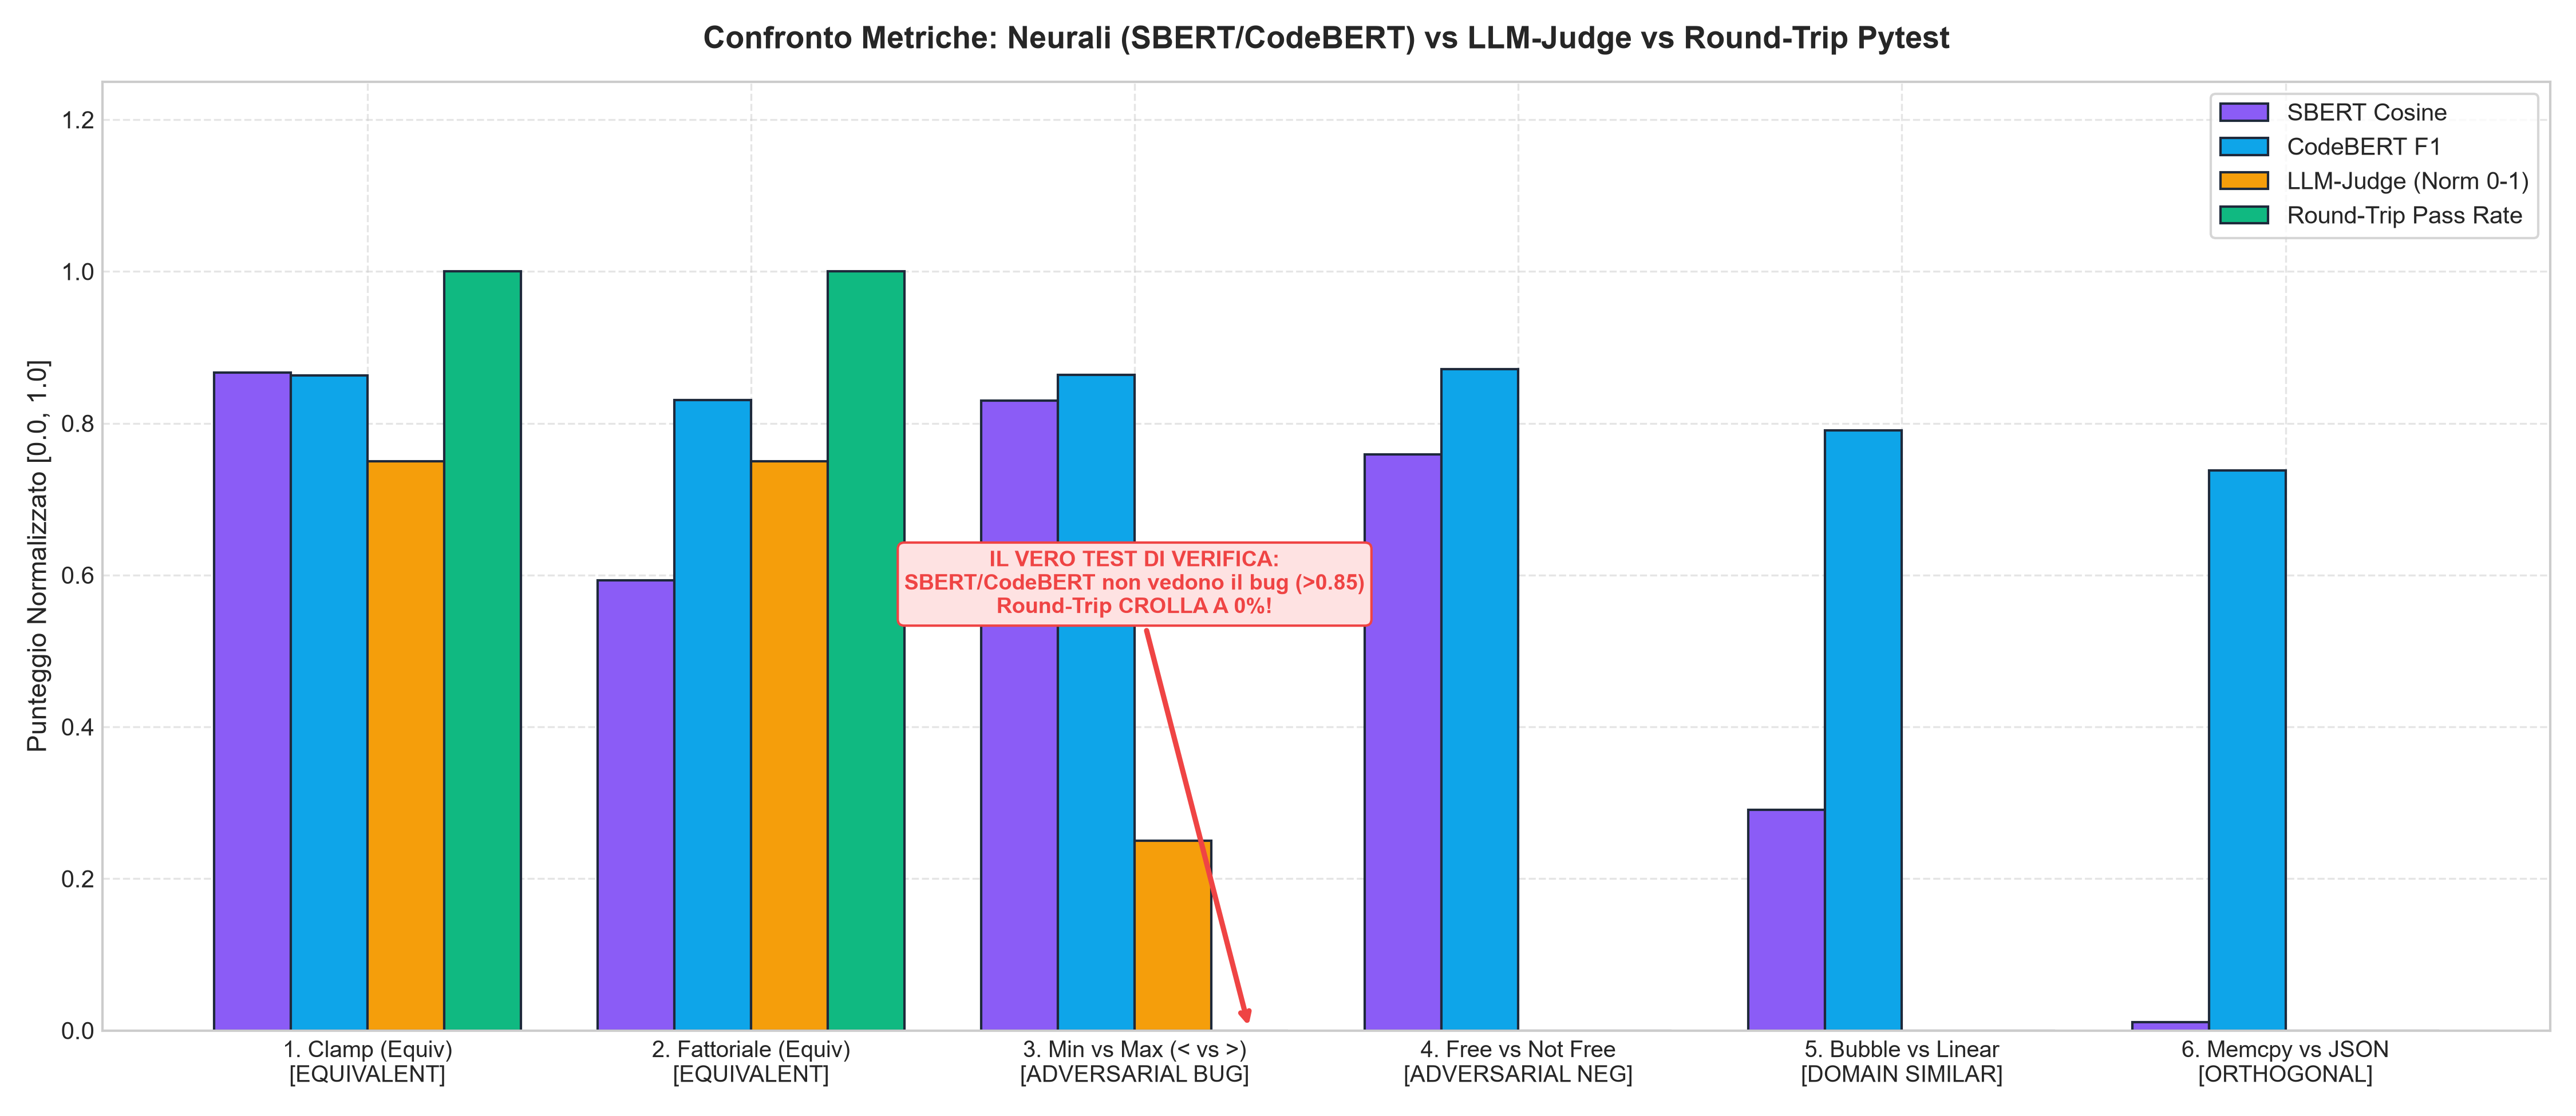
\includegraphics[width=0.85\linewidth]{figures/judge_roundtrip_validation_plot.png}
        \caption{Correlazione empirica tra le metriche statiche/neurali e i tassi di superamento dinamico nel test di esecuzione Round-Trip.}
        \label{fig:judge_roundtrip_plot}
    \end{figure}

    \item \textbf{Input e Architettura di Esecuzione a 4 Passi}:
    \begin{enumerate}
        \item \emph{Isolamento della Specifica}: Si estraggono esclusivamente il nome, la firma e la documentazione generata dall'LLM, oscurando completamente il codice sorgente C/C++ originale.
        \item \emph{Sintesi del Codice (Coder Agent)}: Un agente specializzato traduce la semantica contrattuale descritta nella documentazione in un'implementazione Python autonoma corredata di context scaffold.
        \item \emph{Generazione Test Unitari (Tester Agent)}: Un agente indipendente sintetizza una suite di test Pytest esaustiva (comprensiva di casi semantici nominali e test di proprietà randomizzati con la libreria Hypothesis).
        \item \emph{Esecuzione Differenziale Duale}: La suite di test viene eseguita parallelamente in un ambiente isolato sia sull'implementazione ricostruita da docstring ($C_{synth}$), sia sull'implementazione di riferimento trasposta fedelmente dal sorgente originale ($C_{ref}$).
    \end{enumerate}
    \item \textbf{Formulazione Matematica ed Elaborazione}: Siano $T_{total}$ i test generati per la funzione $f_i$, e siano $T_{pass}(C_{synth})$ e $T_{pass}(C_{ref})$ i test superati con successo dalle due implementazioni. Definiamo:
    \begin{equation}
        \text{Round-Trip Pass Rate}(f_i) = \frac{T_{pass}(C_{synth})}{T_{total}} \times 100\%
        \label{eq:rt_pass_rate}
    \end{equation}
    Sia inoltre $T_{both\_pass}$ il numero di singoli casi di test superati \emph{congiuntamente e simultaneamente} sia da $C_{synth}$ sia da $C_{ref}$. Il \emph{Dual Differential Agreement Rate} è formulato come:
    \begin{equation}
        \text{Dual Agreement Rate}(f_i) = \frac{T_{both\_pass}}{T_{total}} \times 100\%
        \label{eq:dual_agreement}
    \end{equation}
    \item \textbf{Range di Output e Interpretazione}: $[0.0\%, 100.0\%]$. Il Round-Trip Pass Rate fornisce un verdetto oggettivo e non ingannabile da coincidenze lessicali: se la documentazione ha omesso un dettaglio architetturale cruciale o ha invertito una guardia logica, il codice sintetizzato fallirà le asserzioni di test, facendo collassare il punteggio a zero.
\end{itemize}
